\documentclass[tikz]{standalone}


\usepackage{tikz}
\usetikzlibrary{calc}
\usepackage{amsmath}
\begin{document}

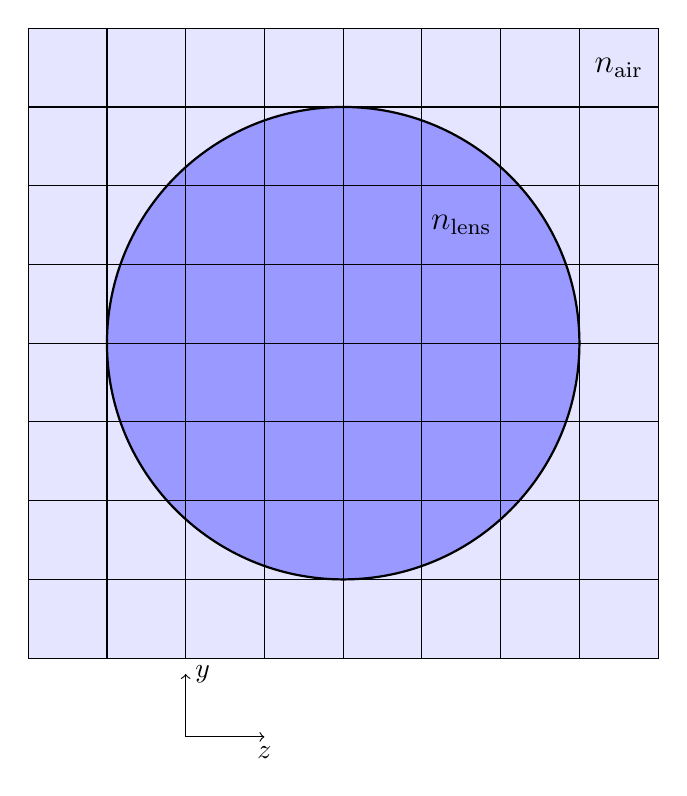
\begin{tikzpicture}
  \draw[fill=blue!10!white] (-4, -4) rectangle (4, 4);
  \draw[thick, fill=blue!40!white] (0,0)  circle (3);
  \node at (3.5,3.5) {\large $n_\text{air}$};
  \node at (1.5,1.5) {\large $n_\text{lens}$};

  \foreach \i in {-4, -3, -2, -1, 0, 1, 2, 3, 4}
  {
    \draw[-] (-4, \i) -- (4, \i);
    \draw[-] (\i, -4) -- (\i, 4);
  }  

  \draw[->] (-2, -5) -- (-1, -5) node [right, below] {$z$};
  \draw[-> ](-2, -5) -- (-2, -4.2) node [right, right] {$y$};

\end{tikzpicture}
\end{document}
